\documentclass[border=6pt]{standalone}
\usepackage{tikz}
\usetikzlibrary{arrows.meta,positioning,calc,shapes.geometric,fit,backgrounds,patterns,matrix,decorations.pathreplacing}
\begin{document}
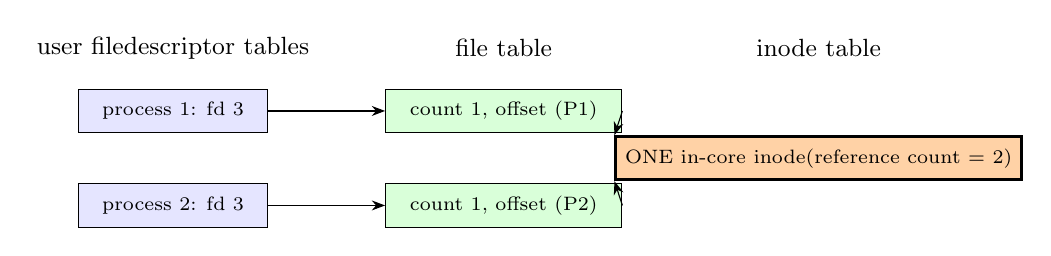
\begin{tikzpicture}[>=Stealth,font=\small]
\tikzstyle{b}=[draw,minimum height=0.55cm,minimum width=2.4cm,font=\scriptsize]
\node[font=\small] at (0,1.9) {user file\\ descriptor tables};\node[font=\small] at (4.2,1.9) {file table};\node[font=\small] at (8.2,1.9) {inode table};
\node[b,fill=blue!10] (u1) at (0,1.1) {process 1: fd 3}; \node[b,fill=blue!10] (u2) at (0,-0.1) {process 2: fd 3};
\node[b,fill=green!15,minimum width=3cm] (f1) at (4.2,1.1) {count 1, offset (P1)}; \node[b,fill=green!15,minimum width=3cm] (f2) at (4.2,-0.1) {count 1, offset (P2)};
\node[b,fill=orange!35,line width=1pt] (i) at (8.2,0.5) {ONE in-core inode\\ (reference count = 2)};
\draw[->] (u1) -- (f1); \draw[->] (u2) -- (f2); \draw[->] (f1.east) -- (i.north west); \draw[->] (f2.east) -- (i.south west);
\end{tikzpicture}
\end{document}
